%! suppress = EscapeHashOutsideCommand
%! Author = Theodore Capinski
%! Date = 4/7/2024

% Preamble
\documentclass[11pt]{article}
\let\oldsection\section
\renewcommand\section{\clearpage\oldsection}
\setcounter{section}{-1}
\counterwithin{figure}{section}

% Packages
\usepackage{amsmath}
\usepackage{hyperref}
\usepackage{graphicx}
\usepackage{tikz}
\usepackage{indentfirst}
\usepackage{calc}
\usepackage{float}

%%%%%%%%%%%%%%%%%%%%%%%%%%%%%%%%%%%%%%%%%%%%%%%%%%%%%%%%%%%%%%%%%%%%%%
% LaTeX Overlay Generator - Annotated Figures v0.0.1
% Created with http://ff.cx/latex-overlay-generator/
%%%%%%%%%%%%%%%%%%%%%%%%%%%%%%%%%%%%%%%%%%%%%%%%%%%%%%%%%%%%%%%%%%%%%%
%\annotatedFigureBoxCustom{bottom-left}{top-right}{label}{label-position}{box-color}{label-color}{border-color}{text-color}
\newcommand*\annotatedFigureBoxCustom[8]{\draw[#5,thick,rounded corners] (#1) rectangle (#2);\node at (#4) [fill=#6,thick,shape=circle,draw=#7,inner sep=2pt,font=\sffamily,text=#8] {\textbf{#3}};}
%\annotatedFigureBox{bottom-left}{top-right}{label}{label-position}
\newcommand*\annotatedFigureBox[4]{\annotatedFigureBoxCustom{#1}{#2}{#3}{#4}{white}{white}{black}{black}}
\newcommand*\annotatedFigureText[4]{\node[draw=none, anchor=south west, text=#2, inner sep=0, text width=#3\linewidth,font=\sffamily] at (#1){#4};}
\newenvironment {annotatedFigure}[1]{\centering\begin{tikzpicture}
                                                   \node[anchor=south west,inner sep=0] (image) at (0,0) { #1};\begin{scope}[x={(image.south east)},y={(image.north west)}]}{\end{scope}\end{tikzpicture}}
%%%%%%%%%%%%%%%%%%%%%%%%%%%%%%%%%%%%%%%%%%%%%%%%%%%%%%%%%%%%%%%%%%%%%%

\newcommand{\todo}[1]{\textcolor{red}{TODO: #1}\PackageWarning{TODO:}{#1!}}

\title{Physics 5BL Lab Report Faradays Law}
\author{T.~Capinski \and A.~Patel}

% Document
\begin{document}
    \maketitle
    \tableofcontents

    \section*{Introduction}\label{sec:introduction}
    \addcontentsline{toc}{section}{Introduction}

    In this lab we did 3 experiments to verify Faradays Law. 
    
    In the first part, we created a generator using the Earth's magnetic field. todo part 1 results
    
    In the second part, we verified Faradays Law by creating a solenoid and measuring the induced current. This part was selected as a summary section and will be mentioned again briefly later in the report.
    
    In the third part, we built a motor using the Earth's magnetic field. This part was selected as a summary section and will be mentioned again briefly later in the report.


    \section*{Theory}\label{sec:theory}
    \addcontentsline{toc}{section}{Theory}


    \section{Part 1: Creating a Generator with the Earth’s Field}\label{sec:part_1}

    \subsection{Methods}\label{subsec:part_1_methods}
    To create a generator using the Earth's magnetic field, we used the setup shown in Figure~\ref{fig:part_1_setup}.

    We hung the IOLab from a spring and coiled magnet wire around it.
    We then connected the wire to the IOLab and rotated the IOLab around the y-axis.
    The IOLab then began simple harmonic motion, which caused the wire to move through the Earth's magnetic field.
    This induced a current in the wire.
    We then measured the induced current and the angular velocity of the IOLab.
    As per the lab notebook, we ran it for over a minute.

    A quick check of the recorded voltage (High Gain on the IOLab) showed a quick oscillation enveloped by a slower oscillation, with amplitude decaying proportional to the spring decay.
    This is shown below in Figure~\ref{fig:high_gain}.

    \begin{figure}[H]
        \centering
        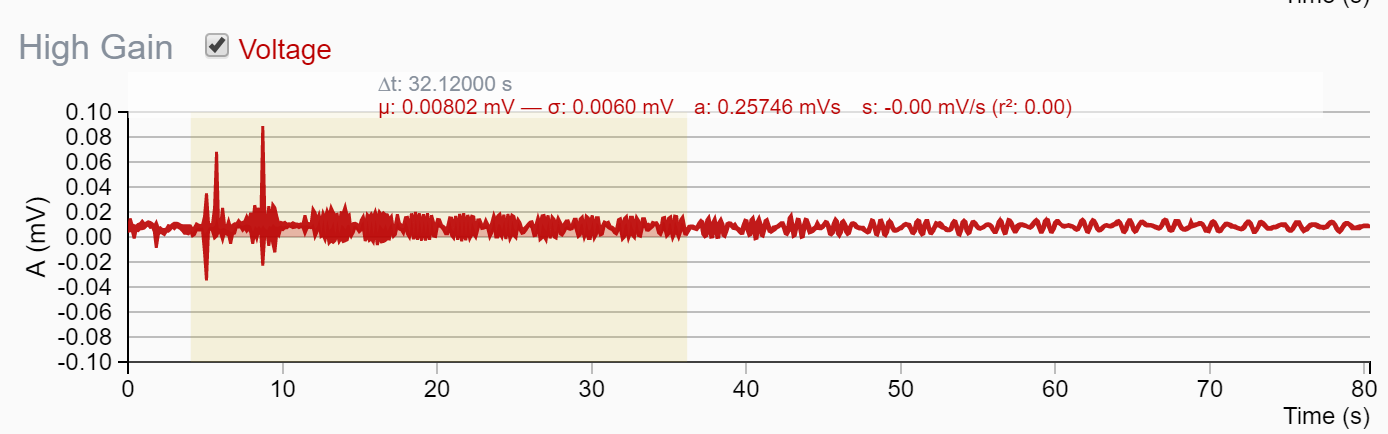
\includegraphics[width=0.8\linewidth]{resources/images/high gain check}
        \caption{Graph of the high gain vs time.}
        \label{fig:high_gain}
    \end{figure}

    \begin{figure}
        \centering
        \begin{annotatedFigure}
        {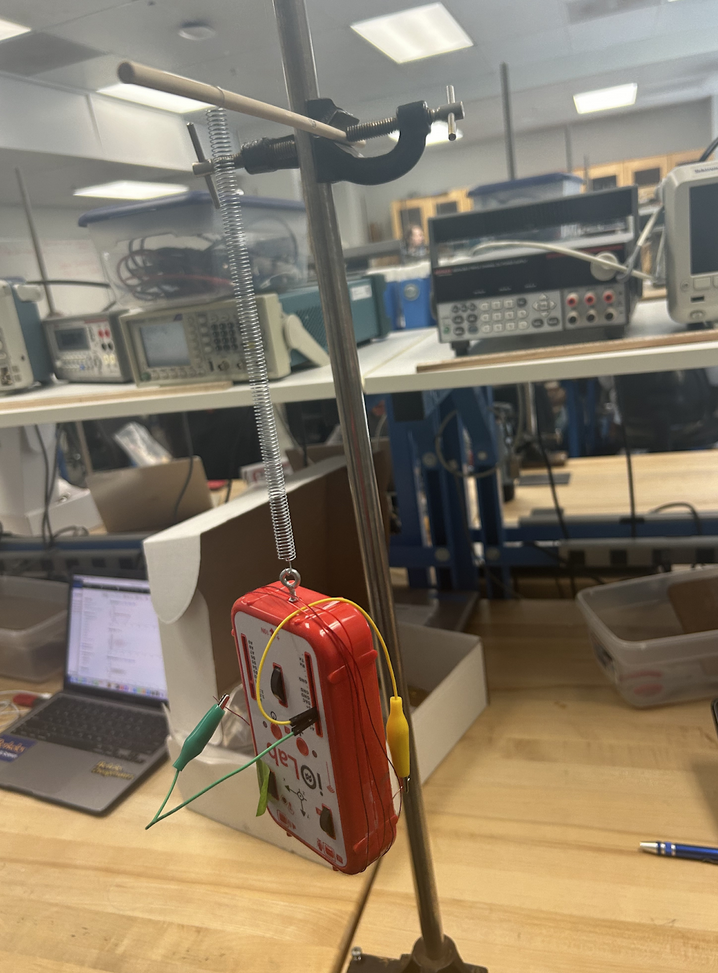
\includegraphics[width=1.0\linewidth]{resources/images/part 1 setup}}
            \annotatedFigureBox{0.1672,0.433}{0.4772,0.826}{A}{0.1672,0.433}%bl
            \annotatedFigureBox{0.2956,0.202}{0.4066,0.327}{B}{0.2956,0.202}%bl
            \annotatedFigureBox{0.0889,0.86}{0.6288,0.95}{C}{0.0889,0.86}%bl
            \annotatedFigureBox{0.2358,0.1319}{0.5855,0.392}{D}{0.2358,0.1319}%bl
        \end{annotatedFigure}
        \caption{Setup for part 1. (A) shows the spring, (b) shows the wiring, (c) shows the dowel, and (d) shows the IOLab with the coiled around it.}
        \label{fig:part_1_setup}
    \end{figure}

    \subsection{Analysis}\label{subsec:part_1_analsysis}

    We expect the induced EMF to be proportional to the angular velocity of the IOLab.
    \todo{from equation something something}
    Using this relationship, we can determine the magnitude of the magnetic field parallel to the Earth's surface at our location.

    First, we graph the induced EMF vs the angular velocity of the IOLab.
    This is shown in Figure~\ref{fig:part_1_graph}.

    \begin{figure}[H]
        \centering
        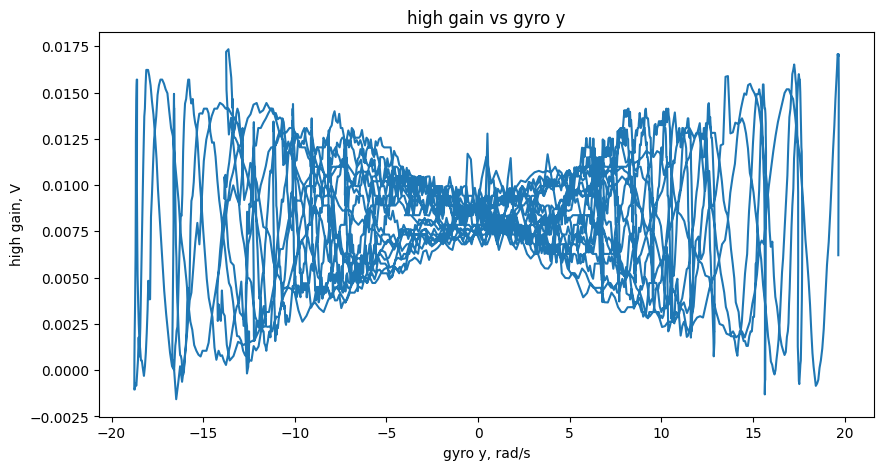
\includegraphics[width=0.8\linewidth]{resources/images/part 1 graph}
        \caption{Graph of the induced EMF vs the angular velocity of the IOLab.}
        \label{fig:part_1_graph}
    \end{figure}

    From this graph, we can determine the slope of the line, which should be equal to the magnitude of the magnetic field parallel to the Earth's surface at our location.

    First, we identify the peaks and troughs of the envelope.

    \begin{figure}[H]
        \centering
        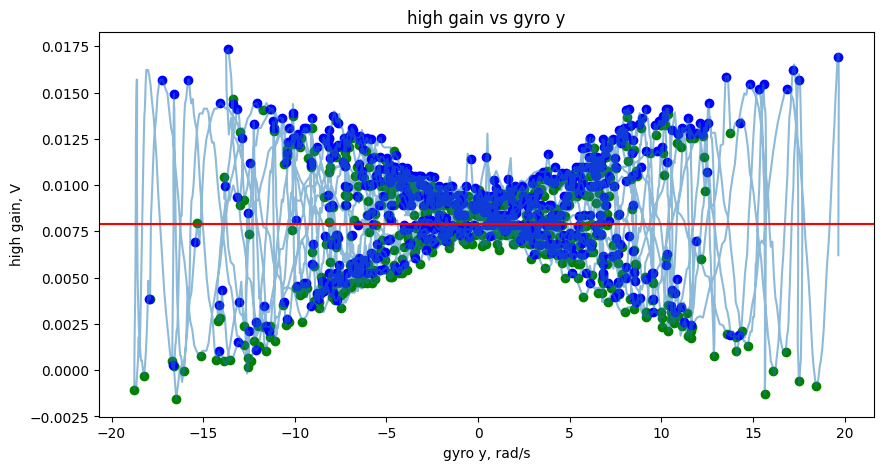
\includegraphics[width=0.8\linewidth]{resources/images/part 1 peaks}
        \caption{Graph of the peaks and troughs of the envelope.}
        \label{fig:part_1_peaks_and_troughs}
    \end{figure}

    For completeness, we will find the slope of both the top-to-bottom and bottom-to-top lines.
    To get the first line, we take the peaks from the first half and the troughs from the second half.
    The second line is the opposite.
    We then fit each line to a linear model and find the slope.
    The average of these two slopes should be the magnitude of the magnetic field parallel to the Earth's surface at our location.

    \begin{figure}[H]
        \centering
        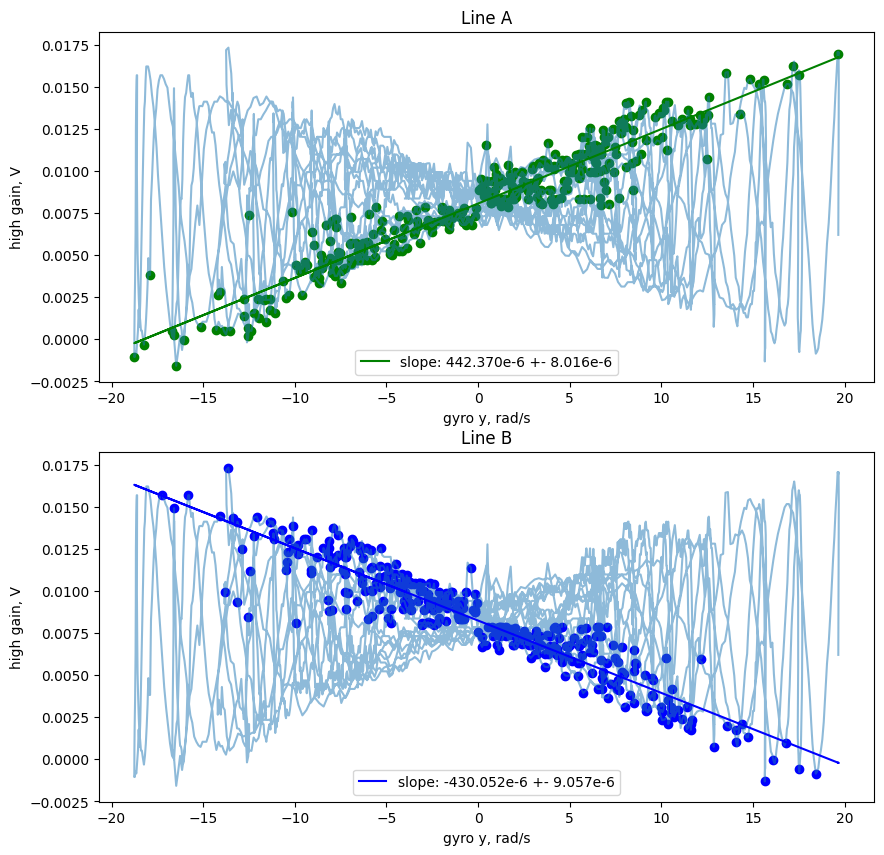
\includegraphics[width=0.8\linewidth]{resources/images/part 1 slopes}
        \caption{Graph of the slopes of the top-to-bottom and bottom-to-top lines.}
        \label{fig:part_1_slopes}
    \end{figure}

    This results in a slope of $442.370e-6 \pm 8.016e-6$ V/(rad/s) and $-430.052e-6 \pm 9.057e-6$ V/(rad/s).

    \subsection{Conclusion}\label{subsec:part_1_conclusion}


    \section{Part 2: Verifying Faraday’s Law (summary section)}\label{sec:part_2}

    For this part, we verified Faradays Law by creating a "solenoid" out of wire and measuring the magnetic field and induced current in the coil. To induce a current, we needed a changing B-field, achieved by moving a magnet up and down directly vertical to the center of the coil, which was placed right on top of the IOlabs magnetar. The setup is shown in the following picture:

    todo: setup part 2
    caption: part 2 setup

    We then plotted the high gain vs the magnetometer and got the following graph:

    todo: high gain vs magnetometer graph
    caption: part 2 graph of high gain (mv) vs magnetometer (µT)

    From this graph, we can see that our data looks similar to the sample data given, especially at the extrema. While our data is slightly more noisy, we can see the general shape is approximately even to the sample.

    Our experiment effectively verified Faraday’s Law by demonstrating the induction of a current in a coil due to a changing magnetic field.  While there was no data analysis done, we can see that our data is qualitatively similar to the example data. The general trend closely resembled the expected behavior, which reaffirms the fundamental principle of electromagnetic induction and underscores its practical relevance in generating electric currents.

    \section{Part 3: Building a Motor (summary section)}\label{sec:part_3}
    In this part, we attempted to create a motor that transforms electrical energy into kinetic energy. This motor uses a stationary magnet that acts as our magnetic field. We then set two conductors on either side of the magnet and a coil of wire with terminals that can reach out and rest in the conductors. This allows current to flow while also allowing the wire coil to rotate. We then connected one side of a battery to each conductor. 

    One of the most important parts of this setup was to only strip part of the coil. On one side, all of the coil needed to be stripped. However, on the other, only one half should be stripped in order to prevent the coil from decelerating itself during the other half-induced current. This took a lot of work and playing around with, but we finally achieved the following setup:

    todo: setup pic part 3
    caption: Setup for part 3

    Using this setup, we were able to take the following video of our motors motion:

    todo: faraday vid 1
    caption: video of motion of built motor

    We then were able to change the direction of the motor by switching the terminals the battery was connected to, and increase the speed by moving the coil closer to the magnet, as shown in the following video:

    todo: faraday vid 2
    caption: video of motion of built motor with increased speed and revered direction

    From these experiments, we can see that by carefully arranging the setup and adjusting parameters such as the position of the coil and the direction of the current flow, we were able to successfully convert electrical energy into kinetic energy. The motion of the motor demonstrates the principles of electromagnetic induction, where the changing magnetic field induces a current in the coil, resulting in rotational motion.

    The ability to change the direction of the motor by switching the battery terminals and increasing the speed of the motor by moving the coil closer to the magnet allows for practical application. This versatility allows for practical applications in various systems where reversible and precise motion is required. Fine-tuning such parameters can lead to optimization and efficiency improvements in motor design.
    
    Overall, these experiments showcase the fundamental concepts of electromagnetism and provide valuable insights into the operation and control of electric motors, laying the groundwork for further exploration and innovation in this field.


    \section{Lab Conclusion}\label{sec:lab_conclusion}
    In this lab, we worked in the realm of magnetism and electromagnetic induction, exploring various phenomena and conducting experiments to deepen our understanding. 

    Experiment 1 aimed to test Faraday’s law directly by utilizing the Earth’s magnetic field to induce an electromotive force (EMF) in a coil. By rotating the coil about the y-axis, we observed an induced EMF, which we expected to be proportional to the angular velocity. Through data analysis and comparison with theoretical predictions, we determined the magnitude of the magnetic field parallel to the Earth’s surface at our location. This experiment not only verified Faraday’s law but also demonstrated the practical application of electromagnetic induction.

    In Experiment 2, which was chosen as a summary section, we sought to verify Faraday’s law by detecting a changing magnetic field using a stationary coil attached to the IOLab. By moving a handheld magnet above the coil and measuring the induced EMF, we investigated the relationship between the EMF and the rate of change of the magnetic field. This gave us a qualitative understanding of magnetic induction in a solenoid.

    Experiment 3, also a summary section, involved the task of building a DC motor, harnessing the interaction between current loops and magnetic fields to generate kinetic energy. By constructing a coil of wire and positioning it between stationary magnets, we aimed to create rotational motion. Through iterative design modifications and troubleshooting, we explored strategies to optimize motor performance, including reversing the motor’s direction and increasing its speed by changing the direction of current and moving the coil closer to the magnet. This experiment showcased the practical application of electromagnetic principles in engineering devices.

    In conclusion, this lab provided valuable hands-on experience in exploring magnetism and electromagnetic induction. Through experimentation and analysis, we deepened our understanding of fundamental electromagnetic phenomena and gained insight into their practical applications.

    \appendix
    \section{References}\label{sec:references}

    Lab Manual
\end{document}